\chapter{Task}
\label{ch:task}
Eventually, it is the generic ability to perform every conceivable task that turns a computing device
into a versatile universal tool. Consequently, the issues of modeling and orchestrating of tasks are
fundamental in the design of any OS. Of course, we cannot expect a single fixed
tasking metaphor to be the ideal solution for all possible kinds of systems and modes of use. For
example, different metaphors are probably appropriate in the cases of a closed mainframe system
serving a large set of users in time-sharing mode on the one hand, and of a personal workstation
that is operated by a single user at a high degree of interactivity on the other hand.

In the case of Oberon, we have consciously concentrated on the domain of personal
workstations. More precisely, we have directed Oberon's tasking facilities towards a single-user
interactive personal workstation that is possibly integrated into a local area network.

We start the presentation in Section 3.1 with a clarification of the technical notion of task. In
Section 3.2, we continue with a detailed explanation of the scheduling strategy. Then, in Section
3.3, we introduce the concept of command. And finally, Section 3.4 provides an overview of
predefined system-oriented toolboxes, i.e. coherent collections of commands devoted to some
specific topic. Example topics are system control and diagnosis, display management, and file management.

\section{The Concept of Task}
In principle, we distinguish two categories of tasks in Oberon: Interactive tasks and background
tasks. Loosely speaking, interactive tasks are bound to local regions on the display screen and to
interactions with their contents while, in contrast, background tasks are system-wide and not
necessarily related to any specific displayed entity.

\subsection{Interactive Tasks}
Every interactive task is represented by a so-called viewer. Viewers constitute the interface to
Oberon's display-system. They embody a variety of roles that are collected in an abstract data
type Viewer. We shall give a deeper insight into the display system in Chapter 4. For the moment
it suffices to know that viewers are represented graphically as rectangles on the display screen
and that they are implicit carriers of interactive tasks. Fig \ref{fig:configuration} shows a typical Oberon display
screen that is divided up into seven viewers corresponding to seven simultaneously active interactive tasks.
\begin{figure}
	\centering
	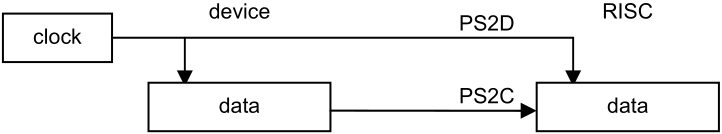
\includegraphics[width=.95\textwidth]{i/3.png}
	\caption{Typical Oberon display configuration with tool track on the right}
	\label{fig:configuration}
\end{figure}

In order to get firmer ground under our feet, we now present the programmed declaration of type Viewer in a slightly abstracted form:
\begin{verbatim}
  Viewer = POINTER TO ViewerDesc;
  ViewerDesc = RECORD
    X, Y, W, H: INT;
    handle: Handler;
    state: INT
  END;
\end{verbatim}
$X$, $Y$, $W$, $H$ define the viewer's rectangle on the screen: location $X$, $Y$ of the lower left corner relative to the display origin, width $W$ and height $H$. The variable state informs about the current state of visibility ($visible$, $closed$, $covered$), while handle represents the functional interface of
viewers. The type of the handler is
\begin{verbatim}
  Handler = PROC(V: Viewer; VAR M: ViewerMsg);
\end{verbatim}
where $ViewerMsg$ is some base type of messages whose exact declaration is of minor importance for the moment:
\begin{verbatim}
  ViewerMsg = RECORD
    ... (*basic parameter fields*)
  END;
\end{verbatim}
However, we should point out the use of object-oriented terminology. It is justified because $handle$ is a procedure variable (a handler) whose identity depends on the specific viewer. A call $V.handle(V, M)$ can therefore be interpreted as the sending of a message $M$ to be handled by the method of the receiving viewer $V$.

We recognize an important difference between the standard object-oriented model and our
handler paradigm. The standard model is closed in the sense that only a fixed set of messages is
understood by a given class of objects. In contrast, the handler paradigm is open because it
defines just the root ($ViewerMsg$) of a potentially unlimited tree of extending message types. For example, a concrete handler might be able to handle messages of type $MyViewerMsg$, where
\begin{verbatim}
  MyViewerMsg = RECORD (ViewerMsg)
    mypar: MyParameters
  END;
\end{verbatim}
is an extended type of $ViewerMsg$.

It is worth noting that our open object-oriented model is extremely flexible. Notably, extending the
set of message types that are handled by an object is a mere implementation issue, that is, it has
no effect at all on the object’s compile-time interface and on the system integrity. It is fair to
mention though that such a high degree of extensibility does not come for free. The price to pay is
the obligation of explicit message dispatching at runtime. The following chapters will capitalize on this property.

Coming back to the perspective of tasks, we note that each sending of a message to a viewer
corresponds to an activation or reactivation of the interactive task that it represents.

\subsection{Background Tasks}
Oberon background tasks are not connected a priori with any specific aggregate in the system.
Seen technically, they are instances of an abstract data type consisting of type declarations $Task$ and $TaskDesc$ together with intrinsic operations $NewTask$, $Install$ and $Remove$:
\begin{verbatim}
  Task = POINTER TO TaskDesc;
  TaskDesc = RECORD
    state: INT;
    handle: PROC
  END;
  PROC NewTask(h: PROC;
               period: INT): Task;
  PROC Install(T: Task);
  PROC Remove (T: Task);
\end{verbatim}
The procedures $Install$ and $Remove$ are called explicitly in order to transfer the state of the specified task from $offline$ to $idle$ and from $idle$ to $offline$ respectively. Installed tasks take their
turns in becoming $active$, that is, in being executed. The installed handlers are simple, parameterless procedures specifying their own actions and conditions for execution, with one exception: Resumption may be delayed until a certain period of time has elapsed. This period is specified in milliseconds when a task is created.

The following two examples of concrete background tasks may serve a better understanding of our explanations. The first one is a system-wide garbage collector collecting unused memory. The second example is a network monitor accepting incoming data on a local area network. In both
examples the state of the task is captured entirely by global system variables. We shall come back to these topics in Chapters 8 and 10 respectively.

We should not end this section without drawing an important conclusion. Transfers of control between tasks are implemented in Oberon as ordinary calls and returns of ordinary procedures (procedure variables, actually). Preemption is not possible. From that we conclude that active periods of tasks are sequentially ordered and can be controlled by a single thread of control. This simplification pays well: Locks of common resources are completely dispensable and deadlocks are not a topic.

\section{The Task Scheduler}
We start from the general assumption that, at any given time, a number of well-determined tasks
are ready in the system to be serviced. Remember that two categories of tasks exist: interactive tasks and background tasks. They differ substantially in the criteria of activation or reactivation
and in the priority of dispatching. Interactive tasks are (re)activated exclusively upon interactions by the user and are dispatched with high priority. In contrast, background tasks are polled with low priority.

We already know that interactive tasks are activated by sending messages. The types of messages used for this purpose are $InputMsg$ and $ControlMsg$ reporting keyboard events and mouse events respectively. Slightly simplified, they are declared as
\begin{verbatim}
  InputMsg = RECORD (ViewerMsg)
    id: INT;
    X, Y: INT;
    keys: SET;
    ch: CHAR
  END;

  ControlMsg = RECORD (ViewerMsg)
    id: INT;
    X, Y: INT
  END;
\end{verbatim}
The field $id$ specifies the exact request transmitted with this specific reactivation. In the case of $InputMsg$ the possible requests are consume (the character specified by field $ch$) and track (mouse, starting from state given by $keys$ and $X$, $Y$). In case of $ControlMsg$ the choice is mark (the viewer at position $X$, $Y$) or neutralize. Mark means moving the global system pointer (typically represented as a star-shaped mark) to the current position of the mouse. Neutralizing a viewer is
equivalent to removing all marks and graphical attributes from this viewer.

All tasking facilities are collected in one module, called Oberon. In particular, the
module's definition exposes the declarations of the abstract data type $Task$ and of the message
types $InputMsg$ and $ControlMsg$. The module's most important contribution, however, is the task
scheduler (often referred to as “Oberon loop”) that can be regarded as the system's dynamic center.

Before studying the scheduler in detail we need some more preparation. We start with the
institution of the focus viewer. By definition, this is a distinguished viewer that by convention
consumes subsequent keyboard input. Note that we identify the focus viewer with the focus task,
hereby making use of the one-to-one correspondence between viewers and tasks.

Module $Oberon$ provides the following facilities in connection with the focus viewer: A global
variable $FocusViewer$, a procedure $PassFocus$ for transferring the role of focus to a new viewer,
and a defocus variant of $ControlMsg$ for notifying the old focus viewer of such a transfer.

The implementation details of the abstract data type $Task$ are hidden from the clients. It is
sufficient to know that all task descriptors are organized in a ring and that a pointer points to the
previously activated task. The ring is guaranteed never to be empty because the above mentioned
garbage collector is installed as a permanent sentinel task at system loading time.

The following is a slightly abstracted version of the actual scheduler code operating on the task
ring. It should be associated with procedure $Loop$ in the module $Oberon$.
\begin{verbatim}
  get mouse position and state of keys;
  REPEAT
    IF keyboard input available THEN read character
      IF character is escape THEN
        broadcast neutralize message to viewers
      ELSIF character is mark THEN
        send mark message to viewer containing mouse
      ELSE send consume message to focus viewer
      END;
      get mouse position and state of keys
    ELSIF at least one key pressed THEN
      REPEAT
        send track message to viewer containing mouse;
        get mouse position and state of keys
      UNTIL all keys released
    ELSE (*no key pressed*)
      send track message to viewer containing mouse;
      take next task in ring as current task;
      call its handler
              (if specified time period has elapsed)
      get mouse position and state of keys
    END 
  UNTIL FALSE
\end{verbatim}
The system executes a sequence of uninterrupted procedures (tasks). Interactive tasks are
triggered by input data being present, either from the keyboard, the mouse, or other input sources.
Background tasks are taken up in a round-robin manner. Interactive tasks have priority.

Having consciously excluded exceptional program behavior in our explanations so far, some
comments about the way of runtime continuation in the case of a failing task or, in other words, in
the case of a trap are in order here. On the (abstract) level of tasks, we can identify three
sequential actions of recovery taken after a program failure:
\begin{verbatim}
  recovery after program failure =
    BEGIN save current system state;
      call installed trap handler;
      roll back to start of task scheduler
    END
\end{verbatim}
Essentially, the system state is determined by the values of all global and local variables at a
given time. The trap handler typically opens an extra viewer displaying the cause of the trap and
the saved system state. Notice in the program fragment above that background tasks are
removed from the ring after failing. This is an effective precaution against cascades of repeated
failures. Obviously, no such precaution is necessary in the case of interactive tasks because their
reactivation is under control of the user of the system.

Summarizing the essence of the tasking system: Oberon is a multitasking system based on a two
category model. Interactive tasks are interfacing with the display system and are scheduled with
high priority upon user interactions. Background tasks are stand-alone and are scheduled with low
priority. Task activations are modeled as message passing and eventually as calls of procedures
assigned to variables. They are sequentially ordered and controlled by a single thread of control.

\section{The concept of command}
An OS constitutes a general purpose platform on which application software
packages can build upon. To software designers the platform appears as interface to "the system"
and (in particular) to the underlying hardware. Unfortunately, interfaces defined by conventional
OSes often suffer from an all too primitive access mechanism that is based solely on
the concept of "software interrupt" or "supervisor call" and on files taking the role of “connecting
pipes". The situation is especially ironic when compared with the development of high-level
programming languages towards extreme abstraction.

We have put greatest emphasis in Oberon on closing the semantic gap between application
software packages and the system platform. The result of our efforts is a highly expressive and
consistent \textbf{application programming interface(API)} in the form of an explicit hierarchy of module
definitions. Perhaps the most significant and most notable outcome of this approach is a collection
of very powerful and system-wide abstract data types like $Task$, $Frame$, $Viewer$, $File$, $Font$, $Text$, $Module$, $Reader$, $Scanner$, $Writer$ etc..

\subsection{Atomic Actions}
The most important generic function of any OS is executing programs. A clarification
of the term program as it is used in Oberon comprises two views: a static one and a dynamic one.
Statically, an Oberon program is simply a package of software together with an entry point. More
formally, an Oberon program is a pair $(M*, P)$, where $M$ is an arbitrary module, $P$ is an exported
parameterless procedure of $M$, and $M*$ denotes the hierarchy consisting of $M$ itself and of all
directly and indirectly imported modules. Note that two hierarchies $M*$ and $N*$ are not generally
disjoint, even if $M$ and $N$ are different modules. Rather, their intersection is a superset of the OS.

Viewed dynamically, an Oberon program is defined as an atomic action (often called command)
operating on the global system state, where atomic means "without user interaction". This
definition is just a necessary consequence of our model of non-preemptive task scheduling with
the benefit of a single carrier thread. We can argue like this: When a traditional interactive
program requires input from the user, , the current task is normally preempted in favor of another
task that produces the required input data. Therefore, a traditional interactive program can be
viewed as a sequence of atomic actions interrupted by actions that possibly belong to other
programs. Whereas in traditional systems these interruptions may occur at any time, in Oberon
they can occur only after the completion of a task, of a command.

Quintessentially, Oberon programs are represented in the form of commands that are in the form
of exported parameterless procedures that do not interact with the user of the system.

Returning to the calling and execution of programs we now arrive at the following refined code version:
\begin{verbatim}
  call program (M*, P) = BEGIN
    load module hierarchy M*;
    call command P
  END
\end{verbatim}
The system interface to the command mechanism itself is again provided by module $Oberon$. Its
primary operation can be paraphrased as "call a command by its name and pass a list of actual parameters":
\begin{verbatim}
  PROC Call (name: ARRAY OF CHAR;
                   par: ParList;
               VAR res: INT);
\end{verbatim}
$name$ is the name of the desired command in the form $M.P$, $par$ is the list of actual parameters,
and $res$ is a result code. But in fact we have separated the setting of parameters from the actual
call. Parameters are set by calling
\begin{verbatim}
  PROC SetPar (F: Display.Frame;
                    T: Texts.Text;
                  pos: INT);
\end{verbatim}
and the actual call is achieved by calling
\begin{verbatim}
  PROC Call (name: ARRAY OF CHAR;
               VAR res: INT);
\end{verbatim}
The pair $(T, pos)$ specifies the starting position of a textual parameter list. $F$ indicates the 
calling viewer. Notice the occurrence of yet another abstract data type of name $Text$ that is exported 
by module $Texts$. We shall devote \ref{ch:text} to a thorough discussion of Oberon's text 
system. For the moment we can simply look at a text as a sequence of characters.

The list of actual parameters is handed over to the called command by module $Oberon$ in the form
of an exported global variable $Par$:
\begin{verbatim}
  Par: RECORD
    vwr  : Viewers.Viewer;
    frame: Display.Frame;
    text : Texts.Text;
    pos  : INT
  END
\end{verbatim}
In principle, commands operate on the entire system and can access the current global state via
the system's powerful abstract modular interface, of which the list of actual parameters is just one
component. Another one is the so-called system log which is a system-wide protocol reporting on
the progress of command execution and on exceptional events in chronological order. The log is
represented as a global variable of type $Text$:
\begin{verbatim}
  Log: Texts.Text;
\end{verbatim}
It should have become clear by now that implementers of commands may rely on a rich arsenal of
abstract global facilities that reflect the current system state and make it accessible. In other
words, they may rely on a high degree of system integration. Therefore, Oberon features an
extraordinarily broad spectrum of mutually integrated facilities. For example, the system
distinguishes itself by a complete integration of the abstract data types $Viewer$ and $Text$ that we
encountered above. They will be the subject of \ref{ch:display} and \ref{ch:text}.

Module $Oberon$ assists the integration of these types with the following conceptual features, of
which the first two are familiar to us already: Standard parameter list for commands, system log,
generic text selection, and generic copy viewer. At this point we should add a word of clarification
to our use of the term "generic". It is synonymous with "interpretable individually by any viewer
(interactive task)" and is typically used in connection with messages or orders whose receiver's
exact identity is unknown.

Let us now go into a brief discussion of the generic facilities without, however, leaving the level of
our current abstraction and understanding.

\subsection{Generic Text Selection}
Textual selections are characterized by a text, a stretch of characters within that text, and a time
stamp. Without further qualification "the text selection" always means "the most recent text selection". It can be obtained programmatically by calling procedure $GetSelection$:
\begin{verbatim}
  PROC GetSelection (VAR text: Texts.Text;
                VAR beg, end, time: LONGINT);
\end{verbatim}
The parameters specify the desired stretch of text starting at position $beg$ and ending at $end-1$ as
well as the associated time stamp. The procedure is implemented in form of a broadcast of a socalled selection message to all viewers. The declaration of this message is
\begin{verbatim}
  SelectionMsg = RECORD (ViewerMsg)
    time: INT;
    text: Texts.Text;
    beg, end: INT
  END;
\end{verbatim}

\subsection{Generic Copy Viewer}
Generic copying is synonymous with reproducing and cloning. It is the most elementary generic
operation possible. Again, a variant of type $ViewerMsg$ is used for the purpose of transmitting
requests of the desired type:
\begin{verbatim}
  CopyMsg = RECORD (ViewerMsg)
    vwr: Viewers.Viewer
  END
\end{verbatim}
Receivers of a copy message typically generate a clone of themselves and return it to the sender via field $vwr$.

Let us now summarize this section: Oberon is an OS that presents itself to its
clients in the form of a highly expressive abstract modular interface that exports many powerful
abstract data types like, for example, $Viewer$ and $Text$. A rich arsenal of global data types and
generic facilities serve the purpose of system integration at a high degree. Programs in Oberon
are modeled as so-called commands, i.e. as exported parameterless procedures that do not
interact with the user. The collection of commands provided by a module appears as its user
interface. Parameters are passed to commands via a global parameter list, registered by the
calling task in the central module $Oberon$. Commands operate on the global state of the system.

\section{Toolboxes}
Modules typically appear in three different forms. The first is one that encapsulates some
data, letting them be accessed only through exported procedures and functions. A good example
is $FileDir$, encapsulating the file directory and protecting it from disruptive access. The
second is used to represent an abstract data type, exporting a type and its associated
operators. Typical examples are $Files$, $Modules$, $Viewers$, and $Texts$. The third is the
collection of procedures pertaining to the same topic, such as $RS232$ handling
communication over a serial line.

Oberon adds a fourth form: the toolbox. By definition, this is a pure collection of commands in the
sense of the previous section. Toolboxes distinguish themselves principally from the other forms
of modules by the fact that they lie on top of the modular hierarchy. Toolbox modules are
"imported" by system users at run-time. In other words, their definitions define the user interface.
Typical examples are $System$ and $Edit$. As a rule of thumb there exists a toolbox for
every topic or application.

As an example of a toolbox definition we quote an annotated version of $System$:
\begin{verbatim}
  DEFINITION System;
    (*System management, Chapter 3 and 8*)
    PROC SetUser;  (*identification*)
    PROC SetFont;  (*for typed text*)
    PROC SetColor; (*for typed text&graphics*)
    PROC SetOffset;(*for typed text*)
    PROC Date;     (*set/get date&time*)
    PROC Collect;  (*garbage*)
    (*Display management, Chapter 4*)
    PROC Open;  (*viewer*)
    PROC Close; (*viewer*)
    PROC CloseTrack;
    PROC Recall;(*most recently closed viewer*)
    PROC Copy;  (*viewer*)
    PROC Grow;  (*viewer*)
    PROC Clear; (*log*)
    (*Module management, Chapter 6*)
    PROC Free;        (*specified modules*)
    PROC ShowCommands;(*of specified module*)
    PROC ShowModules; (*show loaded modules*)
    (*File management, Chapter 7*)
    PROC Directory;
    PROC CopyFiles;
    PROC RenameFiles;
    PROC DeleteFiles;
    (*System inspection, Chapter 8*)
    PROC Watch;(*tasks, memory&disk storage*)
  END System;
\end{verbatim}
An important consequence of our integrated systems approach is the possibility of constructing a
universal, interactive command interpreter bound to viewers of textual contents. If the text obeys
the following syntax (specified in EBNF, Extended Backus-Naur Form), we call it command tool:
\begin{verbatim}
  CommandTool= {
    [Comment] CommandName [ParameterList]
  }
\end{verbatim}
If present, the parameter list is made available to the called command via fields $text$ and $pos$ in
the global variable $Par$ that is exported from $Oberon$. Because this parameter list is
interpreted individually by each command, its format is completely open. However, we postulate
some conventions and rules for the purpose of a standardized user interface:

\begin{enumerate}
	\item The elements of a textual parameter list are universal syntactical tokens like name, literal
string, integer, real number, and special character.
	\item An arrow "\^{}" in the textual parameter list refers to the current text selection for continuation. In
the special case of the arrow following the command name immediately, the entire parameter list
is represented by the text selection.
	\item An asterisk "*" in the textual parameter list refers to the currently marked viewer. Typically, the
asterisk replaces the name of a file. In such a case the contents of the viewer marked by the
system pointer (star) is processed by the command interpreter instead of the contents of a file.
	\item An at-character "@" in the textual parameter list indicates that the selection marks the
(beginning of the) text which is taken as operand.
	\item A terminator-character "\~{}" terminates the textual parameter list in case of a variable number of
parameters.
\end{enumerate}

Because command tools are ordinary, editable texts (in contrast to menus in conventional
systems) they can be customized "on the fly", which makes the system highly flexible. We refer
again to Fig \ref{fig:configuration} that shows a typical Oberon screen layout consisting of two vertical tracks, a
wider user track on the left and a narrow system track on the right. Three documents are
displayed in the user track: A text, a graphic, and a picture. In the system track we find one logviewer displaying the system log, two tool-viewers making available the standard system tool and
a customized private tool respectively.

In concluding this Chapter, let us exemplify the concepts of command and tool by the system control section of the $System$ toolbox. Consisting of the commands $SetUser$, $Date$, $SetFont$, $SetColor$, and $Collect$, it is used to control system-wide facilities. In detail, their function is installing the user's identification, displaying or setting the system date and time, presetting the system type-font for typed text, setting the system color, and activating the garbage collector.

In summary, a toolbox is a special form of an Oberon module. It is defined as a collection of commands. Appearing at the top of the modular hierarchy the toolboxes in their entirety fix the system’s user interface. Command tools are sequences of textually represented command calls. They are editable and customizable. In a typical Oberon screen layout the tools are displayed in viewers within the system track.
